\chapter{Aminen en stikstofverbindingen}\label{ch:b2:amines}

Vis die niet meer vers is, ruikt naar trimethylamine, een klein vluchtig amine.
Een scheutje citroensap neemt de geur weg: het zuur protoneert het amine, en
het gevormde ammoniumion kan, als ion, niet verdampen. Het vrije elektronenpaar van stikstof
maakt aminen tot basen en nucleofielen; gebonden aan een carbonylgroep geeft het \omterm{def:b2:amines:imine}{iminen},
waarlangs eiwitten hun chemie voeren en chemici aminen maken; en op
een \omterm{def:b2:huckel:aromatic}{aromatische} ring opent het, via diazoniumzouten, de weg naar de azokleurstoffen
die de negentiende eeuw kleur gaven.

\begin{recall}
Het deel van jaar~1: zuren en basen volgens Brønsted, $\mathrm pK_a$ en predominantiediagrammen,
nucleofielen en de bimoleculaire substitutie, hemiacetalen en acetalen, hydridedonoren,
organomagnesiumverbindingen, de klasse van een koolstofatoom. \Cref{ch:b2:aromatic-substitution}:
nitrering, de reductie van nitroarenen. Het schoolboek: aminen en amiden.
\end{recall}

\begin{omfigure}
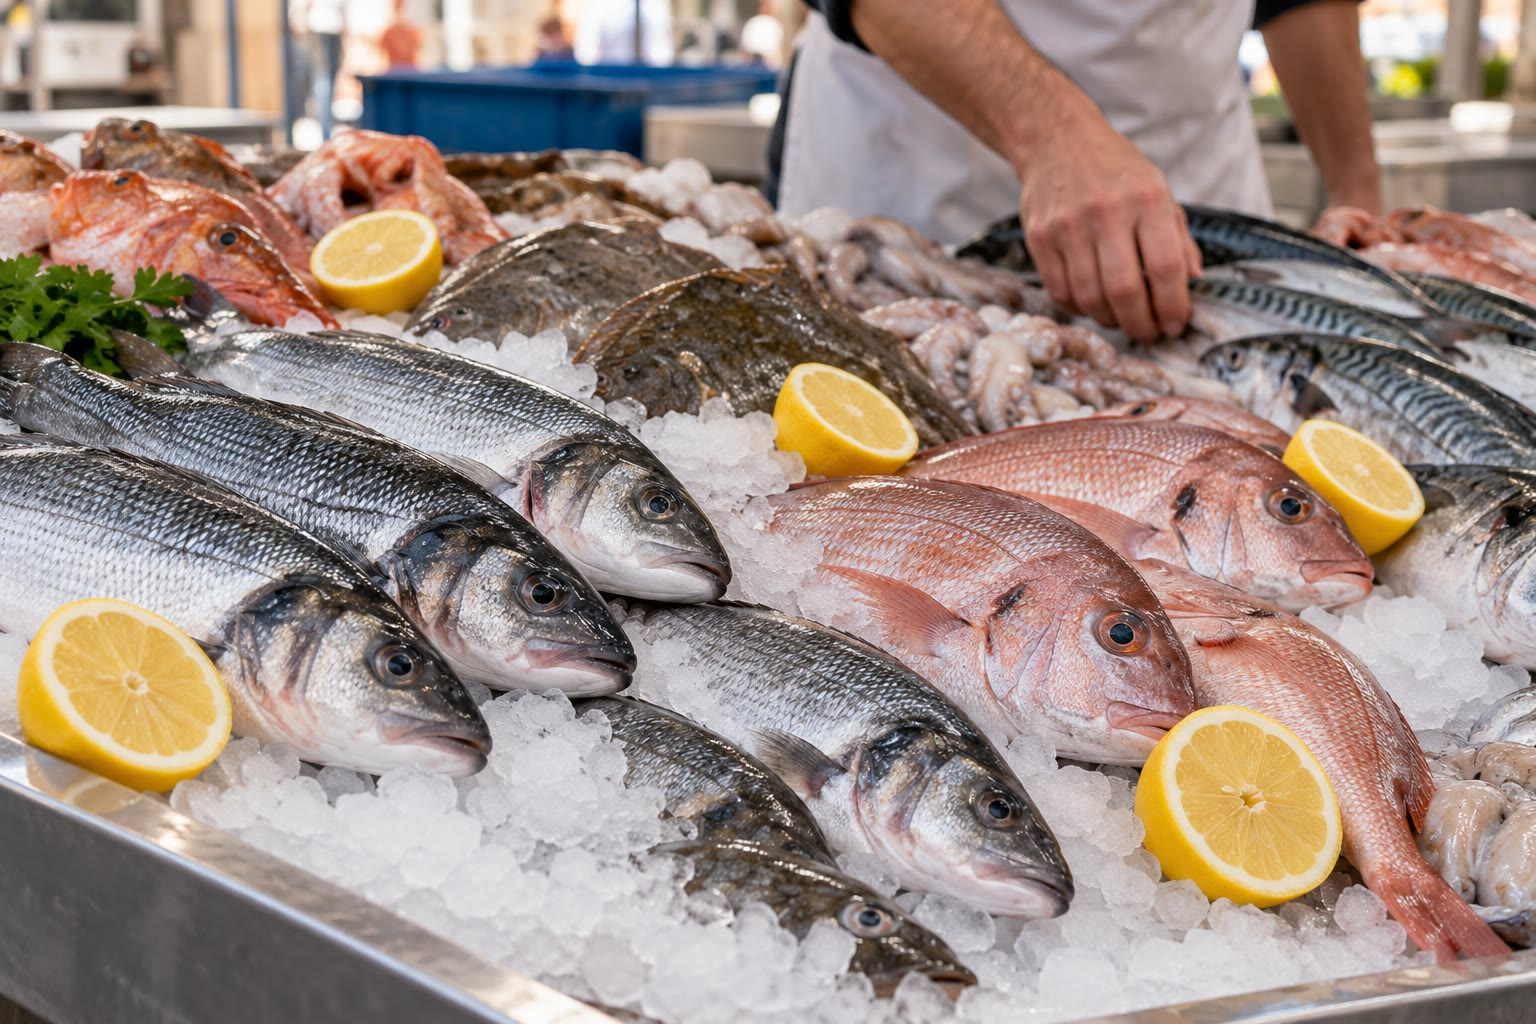
\includegraphics[width=0.6\linewidth]{images/book3/ai/b2-23-fish-stall.jpg}

{\small Een viskraam: tussen de vis liggen gehalveerde citroenen. Hun zuur zet het
trimethylamine van de vis om in zijn niet-vluchtige ammoniumion.}
\end{omfigure}

\section{Structuur en basiciteit}

\begin{definition}[Klassen van aminen]\label{def:b2:amines:class}
Een amine is een \emph{primair amine}\index{primair amine} \ce{RNH2}, een \emph{secundair amine}
\index{secundair amine} \ce{R2NH} of een \emph{tertiair amine}\index{tertiair amine}
\ce{R3N}, naargelang het aantal koolstofgroepen dat aan stikstof gebonden is. Een \emph{quaternair
ammoniumion}\index{quaternair ammoniumion} \ce{R4N+} heeft er vier, en geen vrij elektronenpaar.
\end{definition}

Het stikstofatoom van een amine is ruwweg tetraëdrisch; het vrije elektronenpaar bezet de vierde
positie. Een \omterm{def:b2:amines:class}{tertiair amine} met drie verschillende groepen is in principe chiraal, maar kan niet
gesplitst worden: het molecuul klapt om via een vlakke schikking, als een paraplu in de wind,
duizenden miljoenen keren per seconde bij kamertemperatuur.

\begin{proposition}[Basiciteit]\label{prop:b2:amines:basicity}
In water zijn alkylaminen sterkere basen dan ammoniak ($\mathrm pK_a$ van hun ammoniumionen
rond 10 tot 11, tegenover 9.26), arylaminen veel zwakkere (anilinium 4.60), en amiden nauwelijks
basisch (geprotoneerd ethaanamide ongeveer $-0.6$).
\end{proposition}

\begin{proof}[Redenering]
Alkylgroepen duwen elektronendichtheid naar stikstof (inductief effect) en stabiliseren de
positieve lading van het ammoniumion. In water telt ook de solvatatie door waterstofbruggen: een
ion met meer bindingen \ce{N-H} wordt beter gesolvateerd, en daarom is trimethylammonium (9.80) een
zwakker zuur dan ammonium, maar een sterker dan dimethylammonium (10.73). In aniline is het vrije
elektronenpaar gedelokaliseerd in de ring en gaat het bij protonering verloren; in een amide is het gedelokaliseerd
naar het carbonylzuurstofatoom, en de protonering gebeurt, zwak, op zuurstof.
% ledger: kb:NH3, pka:methylammonium, pka:dimethylammonium, pka:trimethylammonium, pka:anilinium, pka:ethanamideH
\end{proof}

\begin{omfigure}
\begin{tikzpicture}[font=\small, x=0.85cm]
  \draw[->, thick] (-1.5,0) -- (11.8,0) node[below right] {$\mathrm pK_a$};
  \foreach \x in {0,2,4,6,8,10} \draw (\x,0.1) -- (\x,-0.1) node[below, font=\scriptsize] {\x};
  \foreach \x/\l in {-0.6/{\ce{CH3CONH3+}}, 4.60/{\ce{C6H5NH3+}}} {
    \draw[omDef, thick] (\x,0) -- (\x,0.5);
    \node[font=\scriptsize, anchor=south] at (\x,0.5) {\l};
  }
  \foreach \x/\l/\y/\h in {9.26/{\ce{NH4+} (9.26)}/1.95/1.2, 9.80/{\ce{(CH3)3NH+} (9.80)}/1.45/0.85, 10.66/{\ce{CH3NH3+} (10.66)}/0.95/0.5, 10.73/{\ce{(CH3)2NH2+} (10.73)}/0.45/0.25} {
    \draw[omDef, thick] (\x,0) -- (\x,\h);
    \draw[black!40] (\x,\h) -- (12.2,\y);
    \node[font=\scriptsize, anchor=west] at (12.2,\y) {\l};
  }
  \node[font=\scriptsize, anchor=north west] at (-1.4,-0.5) {zwakkere basen};
  \node[font=\scriptsize, anchor=north east] at (11.7,-0.5) {sterkere basen};
\end{tikzpicture}

{\small $\mathrm pK_a$ van de geconjugeerde zuren van enkele stikstofbasen bij
\qty{25}{\degreeCelsius}: hoe hoger, hoe sterker de base.}
% ledger: kb:NH3, pka:methylammonium, pka:dimethylammonium, pka:trimethylammonium, pka:anilinium, pka:ethanamideH
\end{omfigure}

\section{Aminen als nucleofielen}

Aminen vallen halogeenalkanen aan door bimoleculaire substitutie. Het product, een meer gesubstitueerd
amine, is minstens even nucleofiel als het uitgangsamine en concurreert om het halogeenalkaan:
alkylering van ammoniak geeft een mengsel van primaire, secundaire en \omterm{def:b2:amines:class}{tertiaire aminen} en het
quaternaire zout.

\begin{proposition}[Polyalkylering]\label{prop:b2:amines:polyalkylation}
Directe alkylering van ammoniak of van een \omterm{def:b2:amines:class}{primair amine} geeft mengsels; alleen uitputtende alkylering
tot het quaternaire ammoniumzout verloopt zuiver.
\end{proposition}

\begin{proof}[Redenering]
Elke alkylering laat een vrij elektronenpaar achter op een stikstofatoom dat door de nieuwe alkylgroep
elektronenrijker is geworden; het product reageert met het resterende halogeenalkaan met een vergelijkbare snelheid. Pas wanneer
stikstof geen vrij elektronenpaar meer heeft, in \ce{R4N+}, stopt de reeks.
\end{proof}

\omterm{def:b2:amines:class}{Primaire aminen} zonder hun overgealkyleerde verwanten worden langs een omweg gemaakt: via de route
van Gabriel (alkylering van het stikstofatoom van ftaalimide, dat één zuur waterstofatoom draagt, en daarna
vrijzetting van het amine), door reductie van een \omterm{def:b2:amines:nitrile}{nitril}, van een amide of van een nitroverbinding, of door
\omterm{def:b2:amines:reductive-amination}{reductieve aminering} (zie verder).

\section{Iminen en enaminen}

\begin{definition}[Nucleofiele additie]\label{def:b2:amines:nucleophilic-addition}
Een \emph{nucleofiele additie}\index{nucleofiele additie} aan een carbonylgroep is de aanval van
een nucleofiel op het carbonylkoolstofatoom, dat tetraëdrisch wordt, terwijl de $\pi$-binding van \ce{C=O}
een vrij elektronenpaar op zuurstof wordt.
\end{definition}

\begin{definition}[Hemiaminalen, iminen en enaminen]\label{def:b2:amines:imine}
Een \omterm{def:b2:amines:class}{primair amine} addeert aan een aldehyde of een keton en geeft een \emph{hemiaminaal}\index{hemiaminaal}
(een koolstofatoom dat \ce{OH} en \ce{NHR} draagt); de dehydratatie ervan geeft een \emph{imine}\index{imine}
$\mathrm{R_2C{=}NR'}$. Een \omterm{def:b2:amines:class}{secundair amine}, dat geen neutraal imine kan vormen, geeft na dehydratatie een
\emph{enamine}\index{enamine} $\mathrm{R_2C{=}CR{-}NR'_2}$, waarbij de dubbele binding naar het naburige koolstofatoom verschuift.
\end{definition}

\begin{omfigure}
\setchemfig{atom sep=1.9em}
\schemestart
\chemfig{R_2C=O} \+ \chemfig{H_2N-R'}
\arrow{<=>}
\chemfig{R_2C(-[2]OH)-NH-R'}
\arrow{<=>[\ce{H+}][$-$ \ce{H2O}]}
\chemfig{R_2C=N-R'}
\schemestop
\par\vspace{6pt}

{\small Vorming van een \omterm{def:b2:amines:imine}{imine}: \omterm{def:b2:amines:nucleophilic-addition}{nucleofiele additie} van het amine aan de carbonylgroep geeft het
\omterm{def:b2:amines:imine}{hemiaminaal}; zure katalyse maakt van zijn \ce{OH} een vertrekkende groep (\ce{-OH2+}), water vertrekt en
het vrije elektronenpaar van stikstof vormt de dubbele binding \ce{C=N}. Elke stap is omkeerbaar: water in overmaat
hydrolyseert het \omterm{def:b2:amines:imine}{imine} weer terug.}
\end{omfigure}

\begin{proposition}[Optimale pH]\label{prop:b2:amines:imine-ph}
\omterm{def:b2:amines:imine}{Iminen} vormen zich het snelst in licht zure oplossing, rond pH 4 tot 5.
\end{proposition}

\begin{proof}[Redenering]
De eerste stap heeft het vrije amine nodig (zijn vrije elektronenpaar); een te zuur medium protoneert het amine
($\mathrm pK_a$ ongeveer 10) en neemt het nucleofiel weg. De dehydratatie heeft zuur nodig om de
hydroxylgroep te protoneren; bij hoge pH is ze traag. De snelheid, het product van beide behoeften, is het grootst
daartussen.
\end{proof}

\begin{definition}[Reductieve aminering]\label{def:b2:amines:reductive-amination}
Een \emph{reductieve aminering}\index{reductieve aminering} zet een carbonylverbinding en een
amine om in een meer gesubstitueerd amine door het \omterm{def:b2:amines:imine}{imine} (of iminiumion) te vormen en het in dezelfde
pot te reduceren, meestal met natriumcyanoboorhydride \ce{NaBH3CN}.
\end{definition}

\begin{proposition}[Selectiviteit van de reductieve aminering]\label{prop:b2:amines:reductive-amination}
Bij een pH rond 6 reduceert \ce{NaBH3CN} het iminiumion veel sneller dan de carbonylverbinding, zodat
het amine gevormd wordt zonder dat het aldehyde of keton tot een alcohol gereduceerd wordt.
\end{proposition}

\begin{proof}[Redenering]
De cyanogroep maakt van \ce{BH3CN-} een zwakke hydridedonor, te zwak voor een neutrale carbonylgroep maar
voldoende voor een geprotoneerd, positief geladen iminiumion, een veel beter elektrofiel.
\end{proof}

\section{Diazoniumzouten}

\begin{definition}[Diazoniumchemie]\label{def:b2:amines:diazonium}
Een \emph{diazoniumion}\index{diazoniumion} is een kation \ce{R-N+#N}. \emph{Diazotering}\index{diazotering}
zet een primair \omterm{def:b2:huckel:aromatic}{aromatisch} amine om in een aryldiazoniumzout met natriumnitriet en een sterk zuur bij
0--\qty{5}{\degreeCelsius}. Bij een \emph{sandmeyerreactie}\index{sandmeyerreactie} vervangt een koper(I)zout
(\ce{CuCl}, \ce{CuBr}, \ce{CuCN}) de diazoniumgroep door Cl, Br of CN, onder verlies van
distikstof. Bij een \emph{azokoppeling}\index{azokoppeling} valt het diazoniumion, een zwak elektrofiel,
een geactiveerde \omterm{def:b2:huckel:aromatic}{aromatische} ring aan en geeft een azoverbinding $\mathrm{Ar{-}N{=}N{-}Ar'}$.
\end{definition}

\begin{proposition}[Stabiliteit van diazoniumionen]\label{prop:b2:amines:diazonium}
Aryldiazoniumzouten kunnen in koude waterige oplossing bewaard en gebruikt worden; alkyldiazoniumionen verliezen
meteen distikstof.
\end{proposition}

\begin{proof}[Redenering]
Distikstof is een uitstekende vertrekkende groep (een zeer stabiel molecuul, een grote entropiewinst). Bij een
alkylgroep laat het verlies van \ce{N2} een carbokation achter, of valt water rechtstreeks aan: het ion
overleeft niet. Een arylkation is zeer instabiel (een lege $\sigma$-orbitaal in het vlak van de ring,
niet gestabiliseerd door het $\pi$-systeem), en de binding \ce{C-N} van het aryldiazoniumion wordt
versterkt door conjugatie met de ring: bij lage temperatuur blijft het bestaan; opgewarmd ontleedt het,
waarbij water de diazoniumgroep door \ce{OH} vervangt.
\end{proof}

\begin{omfigure}
\begin{tikzpicture}[font=\small, >={Stealth}]
  \node[cyclenode] (d) at (0,0) {\ce{Ar-N2+}};
  \foreach \a/\t/\c in {90/{\ce{Ar-Cl}}/{\ce{CuCl}}, 150/{\ce{Ar-Br}}/{\ce{CuBr}}, 210/{\ce{Ar-CN}}/{\ce{CuCN}},
                        270/{\ce{Ar-OH}}/{\ce{H2O}, warm}, 330/{\ce{Ar-H}}/{\ce{H3PO2}}, 30/{$\mathrm{Ar{-}N{=}N{-}Ar'}$}/{geactiveerd \ce{ArH}}} {
    \node[cyclenode] (p\a) at (\a:2.6) {\t};
    \draw[->, thick] (d) -- (p\a) node[midway, font=\scriptsize, fill=white, inner sep=1pt] {\c};
  }
\end{tikzpicture}

{\small Reacties van een aryldiazoniumzout. De groep \ce{N2+} wordt vervangen door een halogeen of
cyanide (Sandmeyer, koper(I)zouten), door \ce{OH} (warm water) of door H (hypofosforigzuur), of
blijft behouden in een \omterm{def:b2:amines:diazonium}{azokoppeling}.}
\end{omfigure}

\begin{method}[Routes via een diazoniumzout]\label{met:b2:amines:diazonium-routes}
\begin{enumerate}
  \item Gebruik de aminogroep (sterk ortho/para-sturend) om andere groepen te plaatsen, en zet ze daarna
        om via het diazoniumzout.
  \item Vervang ze door H om patronen te verkrijgen die directe substitutie niet kan geven
        (1,3,5-tribroombenzeen uit aniline).
  \item Vervang ze door CN en hydrolyseer daarna tot een carbonzuur: een weg naar \ce{-COOH} op een ring.
\end{enumerate}
\end{method}

\begin{method}[Een amine maken]\label{met:b2:amines:make-amine}
\begin{enumerate}
  \item \omterm{def:b2:amines:class}{Primair amine} op een alkylketen: route van Gabriel, of reductie van een \omterm{def:b2:amines:nitrile}{nitril} (één koolstofatoom
        meer dan het halogeenalkaan waarmee het gemaakt werd) of van een amide.
  \item Secundair of \omterm{def:b2:amines:class}{tertiair amine}: \omterm{def:b2:amines:reductive-amination}{reductieve aminering} van de juiste carbonylverbinding met
        het juiste amine.
  \item \omterm{def:b2:huckel:aromatic}{Aromatisch} amine: nitrering, daarna reductie (ijzer of tin met zuur, of \omterm{def:b2:alkene-redox:hydrogenation}{katalytische
        hydrogenering}).
\end{enumerate}
\end{method}

\section{Nitrilen}

\begin{definition}[Nitril]\label{def:b2:amines:nitrile}
Een \emph{nitril}\index{nitril} is een verbinding \ce{R-C#N}, gemaakt door substitutie van een halogeenalkaan
met cyanide of door een \omterm{def:b2:amines:diazonium}{sandmeyerreactie}.
\end{definition}

\begin{proposition}[Reacties van nitrilen]\label{prop:b2:amines:nitrile}
Een \omterm{def:b2:amines:nitrile}{nitril} wordt, in zuur of in base, gehydrolyseerd tot het amide en daarna tot het carbonzuur; het wordt
door lithiumaluminiumhydride gereduceerd tot het \omterm{def:b2:amines:class}{primaire amine} \ce{RCH2NH2}; een organomagnesiumverbinding
addeert er één keer aan, en hydrolyse van het gevormde \omterm{def:b2:amines:imine}{imine} geeft een keton.
\end{proposition}

\begin{proof}[Redenering]
Het nitrilkoolstofatoom is elektrofiel, zoals een carbonylkoolstofatoom: water (geactiveerd door zuur, of als
hydroxide) addeert eraan en geeft na tautomerie een amide, waarvan de hydrolyse behandeld wordt in
\cref{ch:b2:acyl-substitution}. Hydride addeert twee keer. Een organomagnesiumverbinding addeert één keer
en geeft een imine-anion dat niet verder reageert; water hydrolyseert het \omterm{def:b2:amines:imine}{imine} daarna tot het keton.
\end{proof}

\begin{safety}{\ghs[5mm]{GHS03}\,\ghs[5mm]{GHS06}\,\ghs[5mm]{GHS08}\,\ghs[5mm]{GHS09}}
Aniline en \textit{N},\textit{N}-dimethylaniline zijn giftig bij contact met de huid; natriumnitriet is
giftig en oxiderend; natriumcyanoboorhydride maakt in zuur blauwzuur vrij en moet gebruikt worden
in een zuurkast. Droge diazoniumzouten kunnen ontploffen: ze worden altijd koud gehouden, in oplossing, en meteen
gebruikt.
% ledger: ghs:aniline, ghs:dimethylaniline, ghs:NaNO2, ghs:NaBH3CN, ghs:sulfanilic-acid
\end{safety}

\section{Oefeningen}

\begin{exercise}[$\star$]\label{exo:b2:amines:1}
Geef de klasse van: propaan-1-amine, \textit{N}-methylethaanamine, triethylamine,
tetramethylammoniumchloride, aniline.
\end{exercise}

\begin{exercise}[$\star$]\label{exo:b2:amines:2}
Rangschik naar toenemende basiciteit: ammoniak, methylamine, aniline, ethaanamide.
\end{exercise}

\begin{exercise}[$\star$]\label{exo:b2:amines:3}
Geef het \omterm{def:b2:amines:imine}{imine} dat gevormd wordt uit cyclohexanon en methylamine, en de omstandigheden.
\end{exercise}

\begin{exercise}[$\star$]\label{exo:b2:amines:4}
Geef, uitgaande van benzeendiazoniumchloride, de producten met \ce{CuBr}, \ce{CuCN}, warm water
en fenol in base.
\end{exercise}

\begin{exercise}[$\star\star$]\label{exo:b2:amines:5}
Welke vorm van trimethylamine overheerst bij pH 7, en in welke verhouding? Verklaar de citroen, en hoe een
amine uit een organisch oplosmiddel naar water geëxtraheerd kan worden.
\end{exercise}

\begin{exercise}[$\star\star$]\label{exo:b2:amines:6}
Geef het \omterm{def:b2:amines:imine}{enamine} dat gevormd wordt uit cyclohexanon en pyrrolidine, en leg uit waarom een \omterm{def:b2:amines:class}{secundair amine}
geen \omterm{def:b2:amines:imine}{imine} kan geven.
\end{exercise}

\begin{exercise}[$\star\star$]\label{exo:b2:amines:7}
Bereid \textit{N}-benzylpropaan-2-amine \ce{C6H5CH2NHCH(CH3)2} door \omterm{def:b2:amines:reductive-amination}{reductieve aminering}: geef twee
mogelijke paren reagentia.
\end{exercise}

\begin{exercise}[$\star\star$]\label{exo:b2:amines:8}
Benzonitril reageert met ethylmagnesiumbromide en daarna met waterig zuur. Geef het product.
\end{exercise}

\begin{exercise}[$\star\star$]\label{exo:b2:amines:9}
Schrijf de synthese van Gabriel van hexaan-1-amine op en leg uit waarom ze geen \omterm{def:b2:amines:class}{secundair amine} geeft.
\end{exercise}

\begin{exercise}[$\star\star\star$]\label{exo:b2:amines:10}
Bereid 1,3,5-tribroombenzeen uit aniline.
\end{exercise}

\begin{exercise}[$\star\star\star$]\label{exo:b2:amines:11}
Ontwerp een azokleurstof uit 4-nitroaniline en fenol: schrijf de \omterm{def:b2:amines:diazonium}{diazotering}, de koppeling (positie
en pH) en het product op.
\end{exercise}

\begin{exercise}[$\star\star\star$]\label{exo:b2:amines:12}
Het quaternaire ammoniumhydroxide van \textit{N},\textit{N}-dimethylbutaan-2-amine geeft bij verhitting
vooral but-1-een. Verklaar deze hofmannoriëntatie, tegengesteld aan de regel van Zaitsev uit het deel
van jaar~1.
\end{exercise}

\section{Probleem: methyloranje maken}

\begin{problem}[{Weekendprobleem --- sulfanilzuur en zijn \omterm{def:b2:amines:diazonium}{diazotering}, de \omterm{def:b2:amines:diazonium}{azokoppeling} met
\textit{N},\textit{N}-dimethylaniline, methyloranje als indicator, en het rendement}]
\label{pb:b2:amines:1}
Gegevens: sulfanilzuur (4-aminobenzeensulfonzuur) \ce{C6H7NO3S}; methyloranje, het natriumzout
\ce{C14H14N3NaO3S}; $\mathrm pK_a$ van de zure vorm van methyloranje 3.47. Molaire massa's
(\unit{g/mol}): C 12.011, H 1.008, N 14.007, O 15.999, Na 22.990, S 32.06. Run (gegevens voor de oefening):
\qty{5.00}{g} sulfanilzuur, rendement 80~\%.
% ledger: pka:methylorange, aw:C, aw:H, aw:N, aw:O, aw:Na, aw:S, ghs:sulfanilic-acid, ghs:NaNO2

\medskip
\noindent\textbf{Deel I --- Sulfanilzuur en \omterm{def:b2:amines:diazonium}{diazotering}.}
\begin{enumerate}
  \item Sulfanilzuur bestaat als zwitterion. Teken het.
  \item Waarom wordt het eerst opgelost in een natriumcarbonaatoplossing?
  \item Schrijf de vorming van salpeterigzuur uit natriumnitriet en zoutzuur op.
  \item Schrijf de \omterm{def:b2:amines:diazonium}{diazotering} van het 4-sulfonatoaniliniumion op.
  \item Waarom wordt de reactie uitgevoerd bij 0--\qty{5}{\degreeCelsius}?
  \item Welke hoeveelheid natriumnitriet is nodig voor \qty{5.00}{g} sulfanilzuur?
  \item Waarom wordt op een lichte overmaat nitriet getest, en wordt die vernietigd?
\end{enumerate}

\medskip
\noindent\textbf{Deel II --- De koppeling.}
\begin{enumerate}[resume]
  \item Waarom is \textit{N},\textit{N}-dimethylaniline een goede partner?
  \item Op welke positie van zijn ring valt het \omterm{def:b2:amines:diazonium}{diazoniumion} aan, en waarom?
  \item Schrijf het product op (als sulfonaat).
  \item Waarom wordt de koppeling uitgevoerd in zwak zure en niet in sterk zure oplossing?
  \item Waarom moet de oplossing daarna basisch gemaakt worden om het natriumzout neer te slaan?
  \item Waarom is het \omterm{def:b2:amines:diazonium}{diazoniumion} een zwak elektrofiel, dat alleen met geactiveerde ringen reageert?
\end{enumerate}

\medskip
\noindent\textbf{Deel III --- Een indicator.}
\begin{enumerate}[resume]
  \item Welke kleur heeft methyloranje in base, en in zuur?
  \item Waar neemt het een proton op?
  \item Over welk pH-gebied verandert zijn kleur?
  \item Waarom geeft het uitgebreide geconjugeerde systeem een zichtbare kleur?
  \item Waarom verschuift protonering de absorptie?
\end{enumerate}

\medskip
\noindent\textbf{Deel IV --- Rendement.}
\begin{enumerate}[resume]
  \item Bereken de molaire massa van sulfanilzuur.
  \item Bereken die van methyloranje (natriumzout).
  \item Bereken de gebruikte hoeveelheid sulfanilzuur.
  \item Bereken de theoretische massa methyloranje.
  \item Welke verliezen verklaren een rendement onder 100~\%?
  \item Geef de massa methyloranje die uit \qty{5.00}{g} sulfanilzuur verkregen wordt bij een rendement
        van 80~\%.
\end{enumerate}
\end{problem}
